\documentclass[tikz,border=6pt]{standalone}
\usepackage[T1]{fontenc}
\usepackage[utf8]{inputenc}
\usepackage{pgfplots}
\usepgfplotslibrary{groupplots}
\usetikzlibrary{calc}
\pgfplotsset{compat=1.18}
\begin{document}
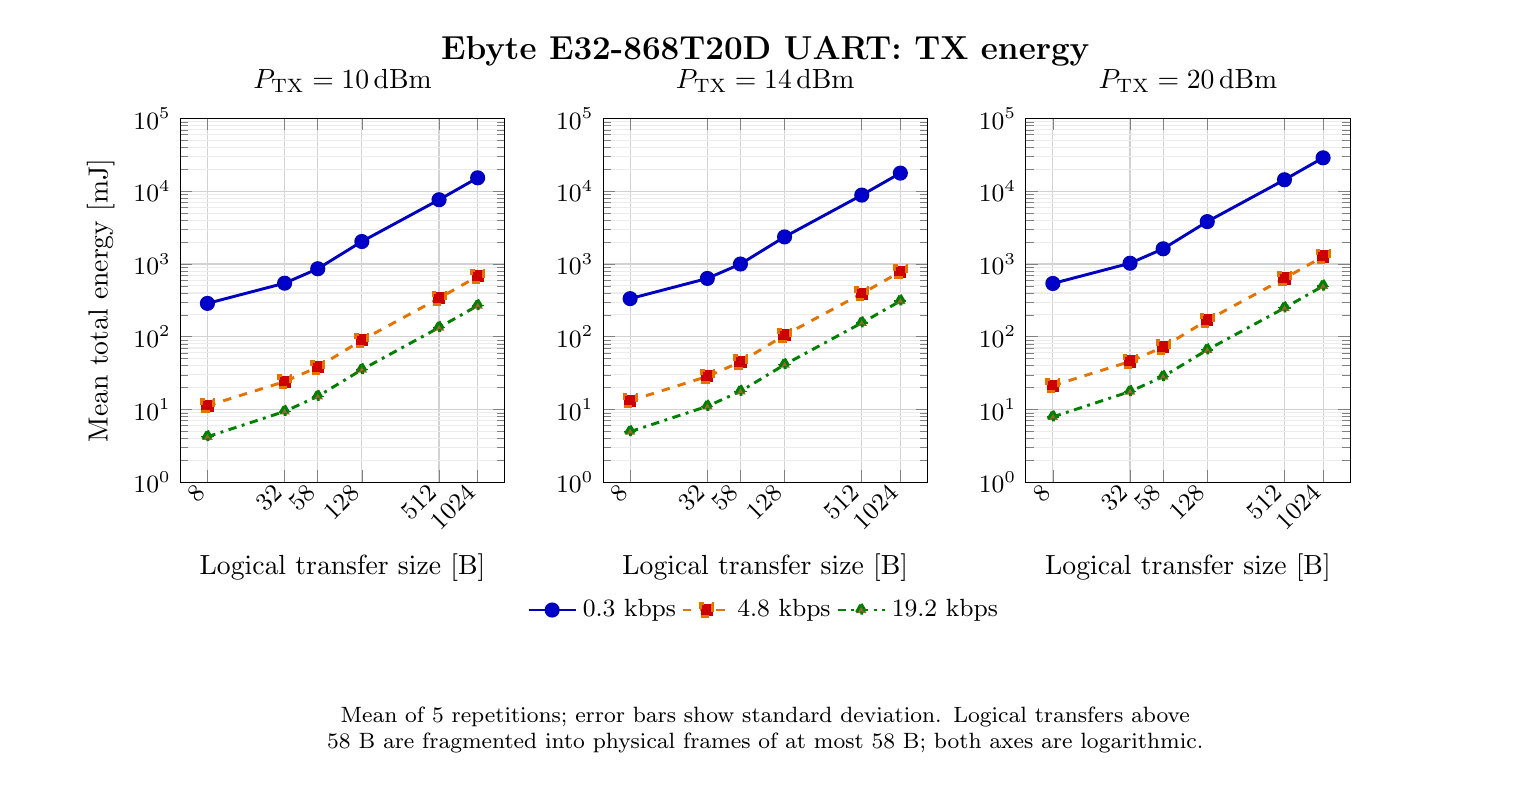
\begin{tikzpicture}
\begin{groupplot}[/pgf/number format/use comma,
  group style={group size=3 by 1, horizontal sep=1.25cm},
  width=5.7cm, height=6.2cm,
  xmode=log, log basis x={2}, ymode=log, log basis y={10},
  ymin=1, ymax=100000,
  xtick={8,32,58,128,512,1024}, xticklabels={8,32,58,128,512,1024},
  x tick label style={rotate=45, anchor=east, font=\small},
  y tick label style={font=\small},
  grid=both, minor grid style={gray!15}, major grid style={gray!35},
  xlabel={Logical transfer size [B]},
  every axis plot/.append style={line width=1.05pt},
  error bars/error bar style={line width=0.35pt},
  legend style={font=\small, draw=none, fill=none, at={(0.5,-0.29)},
    anchor=north, legend columns=-1},
]
\nextgroupplot[title={\(P_{\mathrm{TX}}=10\,\mathrm{dBm}\)}, ylabel={Mean total energy [mJ]}]
\addplot+[
  color=blue!75!black, solid, mark=*, mark size=2.2pt,
  error bars/.cd, y dir=both, y explicit,
] coordinates {
  (8,287.6922) +- (0,0.264202544)
  (32,545.25692) +- (0,0.197897513)
  (58,861.534485) +- (0,0.910123134)
  (128,2040.13856) +- (0,0.830824008)
  (512,7658.45812) +- (0,1.89717351)
  (1024,15329.4489) +- (0,5.32662603)
};
\addplot+[
  color=orange!90!black, dashed, mark=square*, mark size=2.2pt,
  error bars/.cd, y dir=both, y explicit,
] coordinates {
  (8,11.2413954) +- (0,0.0138486911)
  (32,24.1902454) +- (0,0.0258138805)
  (58,38.2279817) +- (0,0.0214650819)
  (128,89.843364) +- (0,0.0720906774)
  (512,338.643049) +- (0,0.127870452)
  (1024,677.510495) +- (0,0.336144427)
};
\addplot+[
  color=green!50!black, dashdotted, mark=triangle*, mark size=2.2pt,
  error bars/.cd, y dir=both, y explicit,
] coordinates {
  (8,4.22021852) +- (0,0.00412012729)
  (32,9.40213564) +- (0,0.0097050617)
  (58,15.1570065) +- (0,0.0119110152)
  (128,35.3144574) +- (0,0.0465270336)
  (512,134.005194) +- (0,0.0588133534)
  (1024,267.818649) +- (0,0.0838755453)
};
\nextgroupplot[title={\(P_{\mathrm{TX}}=14\,\mathrm{dBm}\)}]
\addplot+[
  color=blue!75!black, solid, mark=*, mark size=2.2pt,
  error bars/.cd, y dir=both, y explicit,
] coordinates {
  (8,334.483289) +- (0,0.697986985)
  (32,633.952124) +- (0,0.851263367)
  (58,1000.51615) +- (0,1.19769545)
  (128,2361.26269) +- (0,2.60950586)
  (512,8872.39224) +- (0,9.62156859)
  (1024,17786.5854) +- (0,16.2106868)
};
\addlegendentry{0.3 kbps}
\addplot+[
  color=orange!90!black, dashed, mark=square*, mark size=2.2pt,
  error bars/.cd, y dir=both, y explicit,
] coordinates {
  (8,13.2046357) +- (0,0.0604236531)
  (32,28.5085608) +- (0,0.122548312)
  (58,44.9532863) +- (0,0.157526902)
  (128,105.083758) +- (0,0.52325064)
  (512,392.106646) +- (0,0.598824304)
  (1024,783.097921) +- (0,1.63689386)
};
\addlegendentry{4.8 kbps}
\addplot+[
  color=green!50!black, dashdotted, mark=triangle*, mark size=2.2pt,
  error bars/.cd, y dir=both, y explicit,
] coordinates {
  (8,4.95338168) +- (0,0.0230705382)
  (32,11.0690005) +- (0,0.0443846595)
  (58,17.7584368) +- (0,0.0614366712)
  (128,41.3669793) +- (0,0.218447246)
  (512,155.18176) +- (0,0.504885537)
  (1024,310.37384) +- (0,0.250947326)
};
\addlegendentry{19.2 kbps}
\nextgroupplot[title={\(P_{\mathrm{TX}}=20\,\mathrm{dBm}\)}]
\addplot+[
  color=blue!75!black, solid, mark=*, mark size=2.2pt,
  error bars/.cd, y dir=both, y explicit,
] coordinates {
  (8,540.556196) +- (0,1.27202695)
  (32,1025.92028) +- (0,0.943672525)
  (58,1620.64119) +- (0,2.13478244)
  (128,3832.24699) +- (0,5.7295439)
  (512,14415.9061) +- (0,16.1951417)
  (1024,28883.3701) +- (0,18.9440571)
};
\addplot+[
  color=orange!90!black, dashed, mark=square*, mark size=2.2pt,
  error bars/.cd, y dir=both, y explicit,
] coordinates {
  (8,21.2588305) +- (0,0.0661512523)
  (32,45.7406402) +- (0,0.149573045)
  (58,72.27787) +- (0,0.197643459)
  (128,168.943662) +- (0,0.440621313)
  (512,633.620614) +- (0,0.453536075)
  (1024,1267.55694) +- (0,3.05789592)
};
\addplot+[
  color=green!50!black, dashdotted, mark=triangle*, mark size=2.2pt,
  error bars/.cd, y dir=both, y explicit,
] coordinates {
  (8,7.91021959) +- (0,0.0157846054)
  (32,17.6592511) +- (0,0.068007509)
  (58,28.3587974) +- (0,0.106785966)
  (128,66.0457073) +- (0,0.171066716)
  (512,248.884348) +- (0,0.602431846)
  (1024,498.090636) +- (0,0.436479419)
};
\end{groupplot}
\node[font=\bfseries\large] at ($(group c2r1.north)+(0,0.85cm)$)
  {Ebyte E32-868T20D UART: TX energy};
\node[font=\footnotesize, align=center, text width=18.5cm]
  at ($(group c2r1.south)+(0,-3.15cm)$)
  {Mean of 5 repetitions; error bars show standard deviation. Logical transfers above 58 B are fragmented into physical frames of at most 58 B; both axes are logarithmic.};
\end{tikzpicture}
\end{document}
